\subsection{点的轨迹}\label{subsec:czjh2-7-22}

重物沿着直线自由下落,悬挂着的小锤沿着圆弧往复摆动,在一定的条件之下,
物体沿着一定的轨道运动,这些重物、小锤、物体等运动的轨道,都给我们点的轨迹的形象。

什么是点的轨迹呢?简单地说,点的轨迹就是点按照某个条件运动形成的图形。
符合某个条件的点的轨迹,就是符合某个条件的所有点的集合。
例如,把长度为 $r$ 的线段的一个端点固定,另一个端点绕这个定点旋转一周就得到一个圆。
这个圆上的每一个点,到定点的距离都等于 $r$,同时,到定点的距离等于 $r$ 的所有点,都在这个圆上。
这个圆就叫做到定点的距离等于定长 $r$ 的点的轨迹。

现在,可以给轨迹下定义:

如果下面的两个命题,都是正确的,即

\zhongdian{1. 图形 $F$ 上的每一个点,都符合某个条件 $C$;}

\zhongdian{2. 符合某个条件 $C$ 的每一个点,都在图形 $F$上,}

那么,图形 $F$ 是符合某个条件 $C$ 的\zhongdian{点的轨迹}。

在平面内,这里的图形 $F$ 一般是指某些线。

要注意上面的命题1和2互为逆命题,两者不能互相代替,必须1、2两个命题都是正确的,
图形 $F$ 才是符合条件 $C$ 的点的轨迹,两者缺一不可。

因为原命题和它的逆否命题是等价的,所以上面两个条件也可以说成:
“不符合某个条件 $C$ 的点,都不在图形 $F$上” 和 “不在图形 $F$上的点,都不符合条件 $C$”。

下面,我们讨论一些常见的平面内的点的轨迹。

从上面对圆的讨论,我们知道,圆上的每一点到定点(圆心)的距离都等于定长(半径);
反过来,到定点的距离等于定长的点都在圆上。所以我们可以得出:

\begin{xingzhi}[轨迹1]
    到定点的距离等于定长的点的轨迹,是以定点为圆心,定长为半径的圆。
\end{xingzhi}

在第一册里我们学过,线段垂直平分线上的每一点,和线段两个端点的距离相等;
反过来,和线段两个端点距离相等的点,都在这条线段的垂直平分线上。所以有下面轨迹:

\begin{xingzhi}[轨迹2]
    和已知线段两个端点的距离相等的点的轨迹,是这条线段的垂直平分线。
\end{xingzhi}

由角平分线定理和逆定理,同样可以得到另一个轨迹:

\begin{xingzhi}[轨迹3]
    到已知角两边的距离相等的点的轨迹,是这个角的平分线。
\end{xingzhi}

如果一个动点 $P$ 在平面内运动,它到已知直线 $l$ 的距度始终等于定长 $d$。
我们发现,这个动点运动所形成的图形, 是在 $l$ 两侧的两条平行线 $l'$、$l''$,
它们到 $l$ 的距离都等于 $d$(图 \ref{fig:czjh2-7-81})。

\begin{figure}[htbp]
    \centering
    \begin{minipage}[b]{7cm}
        \centering
        \begin{tikzpicture}
    \pgfmathsetmacro{\b}{1}
    \pgfmathsetmacro{\c}{2.3}
    \pgfmathsetmacro{\d}{4}

    \tkzDefPoints{0/0/A,    \b/0/B,    \c/0/C,    \d/0/D}
    \tkzDefPoints{0/1/A',   \b/1/B',   \c/1/C',   \d/1/D'}
    \tkzDefPoints{0/-1/A'', \b/-1/B'', \c/-1/C'', \d/-1/D''}

    \tkzDrawSegments(A,D  A',D'  A'',D'')
    \tkzLabelSegment[pos=1, right](A,D){$l$}
    \tkzLabelSegment[pos=1, right](A',D'){$l'$}
    \tkzLabelSegment[pos=1, right](A'',D''){$l''$}

    \tkzDrawSegments(B,B''  C,C')
    \tkzLabelSegment[right](B,B''){$d$}
    \tkzLabelSegment[right](C,C'){$d$}
    \tkzMarkRightAngle[size=.2](A,B,B'')
    \tkzMarkRightAngle[size=.2](D,C,C')

    \tkzLabelPoint[above](C'){$P$}
    \tkzLabelPoint[below](B''){$P'$}
\end{tikzpicture}


        \caption{}\label{fig:czjh2-7-81}
    \end{minipage}
    \qquad
    \begin{minipage}[b]{7cm}
        \centering
        \begin{tikzpicture}
    \pgfmathsetmacro{\b}{1.5}
    \pgfmathsetmacro{\c}{4}

    \tkzDefPoints{0/0/A,   \b/0/B,   \c/0/C}
    \tkzDefPoints{0/1/A1,  \b/1/B1,  \c/1/C1}
    \tkzDefPoints{0/-1/A2, \b/-1/B2, \c/-1/C2}

    \tkzDrawSegments(A,C  A1,C1  A2,C2)
    \tkzLabelSegment[pos=1, right](A,C){$l$}
    \tkzLabelSegment[pos=1, right](A1,C1){$l_1$}
    \tkzLabelSegment[pos=1, right](A2,C2){$l_2$}

    \tkzDrawSegments(B,B1  B,B2)
    \tkzLabelSegment[left=.5em](B,B1){$\dfrac{d}{2}$}
    \tkzLabelSegment[left](B2,B){$\exdfrac{d}{2}$}
    \tkzMarkRightAngle[size=.2](A1,B1,B)
    \tkzMarkRightAngle[size=.2](B,B2,C2)

    \tkzLabelPoint[below right](B){$P$}
\end{tikzpicture}


        \caption{}\label{fig:czjh2-7-82}
    \end{minipage}
\end{figure}

因为直线 $l'$、$l''$ 上的每一个点 $P$,到 $l$ 的距离都等于 $d$(夹在两条平行线间的平行线段相等);
反过来,容易证明,如果点 $P'$ 到 $l$ 的距离等于 $d$, 那么点 $P'$ 一定在 $l'$(或 $l''$)上。
这样,我们得到下面轨迹:

\begin{xingzhi}[轨迹4]
    到一条已知直线距离等于定长的点的轨迹,是平行于这条直线,并且到这条直线的距离等于定长的两条直线。
\end{xingzhi}

类似地可以得到:

\begin{xingzhi}[轨迹5]
    到两条平行线距离相等的点的轨迹,是和这两条平行线距离相等的一条平行线
\end{xingzhi}(图 \ref{fig:czjh2-7-82})。

在 \ref{subsec:czjh2-7-5} 节中我们学过,同弧上的圆周角相等。
如图 \ref{fig:czjh2-7-83} 中, $\yuanhu{AMB}$ 和 $\yuanhu{ANB}$ 上每一点,
与 $A$、$B$ 两个端点连线的夹角,都等于已知角;
反过来,在 \ref{subsec:czjh2-7-5} 节例 2 中我们又证明了, 不在 $\yuanhu{AMB}$ 和 $\yuanhu{ANB}$ 上的点与
$A$、$B$ 两点连线的夹角都不等于已知角。于是有下面轨迹:

\begin{xingzhi}[轨迹6]
    和已知线段两个端点连线的夹角等于已知角的点的轨迹,是以已知线段为弦,
    所含圆周角等于已知角的两段弧(端点除外)
\end{xingzhi}(图 \ref{fig:czjh2-7-83})。

要求出同时满足几个条件的点,可以利用上面几个已知轨迹,求满足各个条件的轨迹的交点。

\begin{figure}[htbp]
    \centering
    \begin{minipage}[b]{7cm}
        \centering
        \begin{tikzpicture} % 参考 czjh2-ch7-43
    \pgfmathsetmacro{\a}{45}

    \begin{scope}[xshift=-2cm]
        \tkzDefPoints{0/0/O}
        \tkzDefPoint(0:1.0){A}
        \tkzDefPoint(\a:1.0){B}

        \tkzDrawSegments(O,A  O,B)
        \extkzLabelAngel[0.5](A,O,B){$\alpha$}
    \end{scope}

    \tkzDefPoints{0/0/A, 2.5/0/B}
    \tkzDrawSegment(A,B)
    \tkzLabelPoints[left=.2em](A)
    \tkzLabelPoints[right=.2em](B)

    % 1
    \tkzDefLine[mediator, K=.9](A,B)  \tkzGetPoints{C}{D}

    % 2
    \tkzDefPointBy[rotation=center B angle \a](A)  \tkzGetPoint{e}
    \tkzDefPointOnLine[pos=.5](B,e)  \tkzGetPoint{E}

    % 3
    \tkzDefLine[perpendicular=through B, K=2](E,B)  \tkzGetPoint{F}
    \tkzInterLL(B,F)(C,D)  \tkzGetPoint{O}

    % 4
    \tkzCalcLength(O,A)  \tkzGetLength{rOA}
    \tkzDefShiftPoint[O](60:\rOA){M}
    \tkzDrawArc[thick](O,B)(A)
    \tkzDrawSegments[dashed](A,M  B,M)
    \extkzLabelAngel[0.5](A,M,B){$\alpha$}
    \tkzLabelPoints[above](M)

    % 另一个弧
    \tkzDefPointBy[reflection=over A--B](O)  \tkzGetPoint{O'}
    \tkzDefShiftPoint[O'](-90:\rOA){N}
    \tkzDrawArc[thick](O',A)(B)
    \tkzDrawSegments[dashed](A,N  B,N)
    \extkzLabelAngel[0.5](B,N,A){$\alpha$}
    \tkzLabelPoints[below](N)
\end{tikzpicture}


        \caption{}\label{fig:czjh2-7-83}
    \end{minipage}
    \qquad
    \begin{minipage}[b]{7cm}
        \centering
        \begin{tikzpicture}
    \pgfmathsetmacro{\R}{1.5}

    \begin{scope}[xshift=3.5cm,yshift=3.3cm]
        \tkzDefPoints{0/0/r1, \R/0/r2}
        \tkzDrawSegments[xianduan={below=0pt}](r1,r2)
        \tkzLabelSegment[above](r1,r2){$R$}
    \end{scope}

    \tkzDefPoints{0/0/O, 5/0/A, 2/3.5/B}
    % \tkzDefPoint(50:5){B}
    \tkzDrawSegments(O,A  O,B)
    \tkzLabelPoints[below](A)
    \tkzLabelPoints[left](B,O)

    % 1
    \tkzDefLine[bisector, normed](A,O,B)  \tkzGetPoint{c}
    \tkzDefPointOnLine[pos=5](O,c)  \tkzGetPoint{C}
    \tkzDrawSegment(O,C)
    \tkzLabelPoints[right](C)

    % 2
    \tkzDefShiftPoint[O](90:\R){D}
    \tkzDefLine[parallel=through D](O,A)  \tkzGetPoint{E}
    \tkzDrawSegment(D,E)
    \tkzLabelPoints[left](D)
    \tkzLabelPoints[right](E)

    \tkzInterLL(D,E)(O,C)  \tkzGetPoint{F}
    \tkzLabelPoints[above](F)

    % 3
    \tkzDefShiftPoint[F](270:\R){G}
    \tkzDrawCircle[thick](F,G)
    \tkzDrawSegment(F,G)
    \tkzLabelSegment[right](F,G){$R$}
\end{tikzpicture}


        \caption{}\label{fig:czjh2-7-84}
    \end{minipage}
\end{figure}


\liti[0] 如图 \ref{fig:czjh2-7-84}, 已知 $\angle AOB$。 以已知长 $R$ 为半径,作圆与 $OA$、$OB$ 都相切。

分析:要作符合条件的圆,关键在于确定圆心的位置。

要使圆与 $\angle AOB$ 的两边都相切,这样的圆的圆心的轨迹是 $\angle AOB$ 的平分线;

要使半径等于 $R$ 的圆与 $OA$(或 $OB$)相切,这样的圆心的轨迹是距离 $OA$(或 $OB$)
等于 $R$ 的一条平行线(另一条在角外,不合题意)。

这两个轨迹的交点就是所求圆的圆心。

\zuofa 1. 作 $\angle AOB$ 的平分线 $OC$ (图 \ref{fig:czjh2-7-84})。

2. 作直线 $DE \pingxing OA$, 并且使 $DE$ 与 $OA$ 的距离等于 $R$, $DE$ 与 $OC$ 交于点 $F$。

3. 以 $F$ 为圆心, 以 $R$ 为半径作 $\yuan\,F$。

$\yuan\,F$ 就是所求的圆。

上面的作图可以用来解决一些实际问题。
例如,有两段直路 $l_1$ 和 $l_2$, 它们的位置已经测定,
需要筑一段半径为 $R$ 的圆弧形道路把它们连接起来(图 \ref{fig:czjh2-7-85})。
用上面例题的方法,就可以在图纸上画出这段圆弧 $\yuanhu{AB}$。

\begin{figure}[htbp]
    \centering
    \begin{minipage}[b]{7.5cm}
        \centering
        \begin{tikzpicture} % 参考 czjh2-ch7-84
    \tkzDefPoints{0/0/A, 3/0/a, -1.3/0.6/B, -3/3/b}
    \tkzDrawSegments(A,a B,b)
    \tkzLabelSegment[pos=1, right](A,a){$l_1$}
    \tkzLabelSegment[pos=1, above left](B,b){$l_2$}
    \tkzLabelPoints[below](A)
    \tkzLabelPoints[left](B)

    \tkzInterLL(A,a)(B,b)  \tkzGetPoint{X}
    \tkzDrawSegments[dashed](A,X  B,X)
    % \tkzAutoLabelPoints[center=X, centered, dist= .4](A,B)

    % ---------
    \pgfmathsetmacro{\R}{1.5}

    % 1
    \tkzDefLine[bisector](A,X,B)  \tkzGetPoint{C}

    % 2
    \tkzDefShiftPoint[X](90:\R){D}
    \tkzDefLine[parallel=through D](X,A)  \tkzGetPoint{E}
    \tkzInterLL(D,E)(X,C)  \tkzGetPoint{O}
    \tkzDrawSegments(O,X)
    \tkzDrawPoint(O)
    \tkzLabelPoints[right](O)

    % 3
    \tkzDrawArc(O,B)(A)
    \tkzDrawSegments[-Latex](O,B)
    \tkzLabelSegment[pos=.3, left, yshift=.3em](O,B){$R$}

    % ---------
    \pgfmathsetmacro{\d}{.5}
    \foreach \i in {1,-1} {
        \pgfmathsetmacro{\r}{\R+\i*\d}
        \tkzDefPointOnLine[pos=\r/\R](O,A)  \tkzGetPoint{A'}
        \tkzDefPointOnLine[pos=\r/\R](O,B)  \tkzGetPoint{B'}
        \tkzDrawArc[thick](O,B')(A')


        \tkzDefPointBy[translation=from A to a](A')  \tkzGetPoint{a'}
        \tkzDrawSegment[thick](A',a')

        \tkzDefPointBy[translation=from B to b](B')  \tkzGetPoint{b'}
        \tkzDrawSegment[thick](B',b')
    }
\end{tikzpicture}


        \caption{}\label{fig:czjh2-7-85}
    \end{minipage}
    \qquad
    \begin{minipage}[b]{7cm}
        \centering
        \begin{tikzpicture}
    \pgfmathsetmacro{\R}{2}

    \begin{scope}[xshift=1.2cm,yshift=-2cm]
        \tkzDefPoints{0/0/r1, \R/0/r2}
        \tkzDrawSegments[xianduan={below=0pt}](r1,r2)
        \tkzLabelSegment[above](r1,r2){$R$}
    \end{scope}

    \tkzDefPoints{0/0/O_1, 3.5/0/O_2}
    \tkzDefCircle[R](O_1, 1.5)  \tkzGetPoint{o_1}
    \tkzDefCircle[R](O_2, 1)  \tkzGetPoint{o_2}
    \tkzDrawCircles[thick](O_1,o_1  O_2,o_2)
    \tkzDrawPoints(O_1, O_2)
    \tkzLabelPoints[below](O_1, O_2)
\end{tikzpicture}


        \caption*{(第 2 题)}
    \end{minipage}
\end{figure}


\begin{lianxi}

\xiaoti{说明并作出下列点的轨迹(不要求证明):}
\begin{xiaoxiaotis}

    \xxt{到点 $A$ 的距离等于 5 cm 的点的轨迹;}

    \xxt{半径为 1 cm,并且与半径为 1.5 cm 的圆外切的圆的圆心的轨迹;}

    \xxt{斜边为 $AB$ 的直角三角形的顶点的轨迹;}

    \xxt{经过已知点 $A$ 和 $B$ 的圆的圆心的轨迹;}

    \xxt{半径为 2.5 cm,并且与已知直线 $l$ 相切的圆的圆心的轨迹;}

    \xxt{和两条已知直线 $l_1$ 和 $l_2$ 相切的圆的圆心的轨迹;}

    \xxt{对已知线段 $AB$ 的视角等于 $135^\circ$ 的角的顶点
        (就是使 $\angle APB = 135^\circ$ 的点 $P$)的轨迹。
    }

\end{xiaoxiaotis}


\xiaoti{作半径为 $R$, 并且与已知 $\yuan\,O_1$ 和 $\yuan\,O_2$ 都相外切的圆。}

\end{lianxi}

